\section{An Example Task Walk-through}





To demonstrate the workflow in AnalogSAGE, we use an operational amplifier (op-amp) design task with a set of spec requirements, as shown in Table~\ref{tab:spec_case_study}, which is intentionally designed to be challenging and exceeds the design space in the topology candidates database as an example to illustrate how AnalogSAGE generates a new circuit design.

As shown in Figure~\ref{fig:case_study_refinement}, the \emph{Topology Selection Agent}, equipped with memory from the \emph{Insight Module} and augmented by the \emph{Knowledge Module}, identified an initial topology, which is a two-stage operational amplifier. This topology is then passed to the \emph{Topology Refinement Agent}, which performed no modification and directly forwarded the design to the \emph{Parameter Optimization Agent}, where parameter ranges were estimated and then provided to the \emph{Numerical Module} for numerical optimization. However, the resulting design failed to meet the target specifications, particularly the phase margin. As a failure case in the first iteration, the \emph{Compression Module} analyzed the cause of failure, which in this case was insufficient phase margin, and the \emph{Reflection Module} generated a reflection stating that phase margin must be improved. This feedback was returned to the \emph{Topology Refinement Agent}.

In the second iteration, the \emph{Topology Refinement Agent} received the failure analysis and reflection from the previous iteration and queried the \emph{Knowledge Module} again for improvement suggestions. The retrieved knowledge summarized that introducing Miller compensation would improve phase margin. Following this suggestion, the \emph{Topology Refinement Agent} performed refinement by adding a nulling resistor in series with the Miller capacitor. The modified topology was regenerated as a \texttt{PySpice} \cite{PySpice}  subcircuit and converted into an \texttt{ngspice} \cite{sourceforgeNgspice} compatible netlist, since the LLM is more familiar with Python-based circuit descriptions than raw SPICE syntax. 
% Through iterative optimization in the \emph{Parameter Optimization Agent}, the system identified device parameters whose simulated performance satisfied all target specifications, marking the design as a successfully completed result and it was stored for self-evolving to enhance the ability to solve future design tasks.
Through iterative optimization in the \emph{Parameter Optimization Agent}, the system identified device parameters whose simulated performance satisfied all target specifications. This marked the design as successfully completed. The final result was then stored to support self-evolution and improve performance on future design tasks.

\begin{table}[]
	\centering
	\caption{Spec targets and simulation results in the example.}
	\label{tab:spec_case_study}
	\resizebox{\linewidth}{!}{
		\begin{tabular}{lccc c}
			\hline
			\textbf{Specifications} & \textbf{Unit} & \textbf{Design Target} & \textbf{ AnalogSAGE Result} \\
			\hline
			Gain                    & dB            & $\geq 70$              & 72.88                     \\
			GBW  & Hz            & $\geq 2 \times 10^5$   & 2.4 $\times 10^5$         \\
			Phase Margin            & deg           & $\geq 60$              & 63.80                     \\
			CMRR                    & dB            & $\geq 50$              & 54.57                     \\
			PSRR                    & dB            & $\geq 40$              & 43.88                     \\
			PSRN                    & dB            & $\geq 40$              & 46.55                     \\
			Power                   & $\mu$W        & $\leq 35$              & 30.35                     \\
			\hline
		\end{tabular}}
\end{table}

\begin{figure}[]
	\centering
	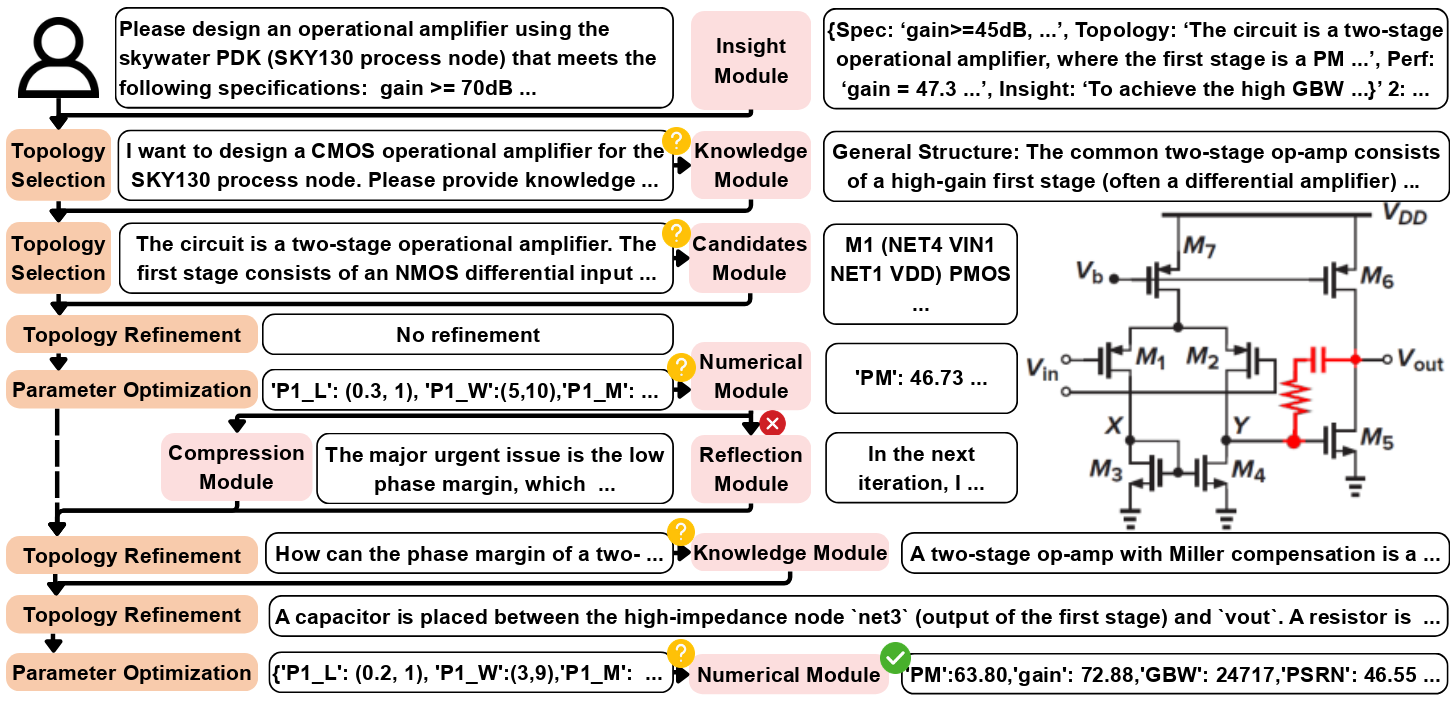
\includegraphics[width=0.45\textwidth]{image/case_study.png}
	\caption{The log of the walk-through example. The refined structure is marked in red, adding Miller compensation with a nulling resistor connected to the output ($\text{V}_{\text{out}}$).}
	\label{fig:case_study_refinement}
\end{figure}

